\documentclass{article}\usepackage[]{graphicx}\usepackage[]{color}
% maxwidth is the original width if it is less than linewidth
% otherwise use linewidth (to make sure the graphics do not exceed the margin)
\makeatletter
\def\maxwidth{ %
  \ifdim\Gin@nat@width>\linewidth
    \linewidth
  \else
    \Gin@nat@width
  \fi
}
\makeatother

\definecolor{fgcolor}{rgb}{0.345, 0.345, 0.345}
\newcommand{\hlnum}[1]{\textcolor[rgb]{0.686,0.059,0.569}{#1}}%
\newcommand{\hlstr}[1]{\textcolor[rgb]{0.192,0.494,0.8}{#1}}%
\newcommand{\hlcom}[1]{\textcolor[rgb]{0.678,0.584,0.686}{\textit{#1}}}%
\newcommand{\hlopt}[1]{\textcolor[rgb]{0,0,0}{#1}}%
\newcommand{\hlstd}[1]{\textcolor[rgb]{0.345,0.345,0.345}{#1}}%
\newcommand{\hlkwa}[1]{\textcolor[rgb]{0.161,0.373,0.58}{\textbf{#1}}}%
\newcommand{\hlkwb}[1]{\textcolor[rgb]{0.69,0.353,0.396}{#1}}%
\newcommand{\hlkwc}[1]{\textcolor[rgb]{0.333,0.667,0.333}{#1}}%
\newcommand{\hlkwd}[1]{\textcolor[rgb]{0.737,0.353,0.396}{\textbf{#1}}}%
\let\hlipl\hlkwb

\usepackage{framed}
\makeatletter
\newenvironment{kframe}{%
 \def\at@end@of@kframe{}%
 \ifinner\ifhmode%
  \def\at@end@of@kframe{\end{minipage}}%
  \begin{minipage}{\columnwidth}%
 \fi\fi%
 \def\FrameCommand##1{\hskip\@totalleftmargin \hskip-\fboxsep
 \colorbox{shadecolor}{##1}\hskip-\fboxsep
     % There is no \\@totalrightmargin, so:
     \hskip-\linewidth \hskip-\@totalleftmargin \hskip\columnwidth}%
 \MakeFramed {\advance\hsize-\width
   \@totalleftmargin\z@ \linewidth\hsize
   \@setminipage}}%
 {\par\unskip\endMakeFramed%
 \at@end@of@kframe}
\makeatother

\definecolor{shadecolor}{rgb}{.97, .97, .97}
\definecolor{messagecolor}{rgb}{0, 0, 0}
\definecolor{warningcolor}{rgb}{1, 0, 1}
\definecolor{errorcolor}{rgb}{1, 0, 0}
\newenvironment{knitrout}{}{} % an empty environment to be redefined in TeX

\usepackage{alltt}
%\usepackage{media9}

\title{Epidemiology -- Human and Water Borne Illnesses}
\author{Marc Los Huertos}
\IfFileExists{upquote.sty}{\usepackage{upquote}}{}
\begin{document}

\maketitle

COVID-19 began spreading rapidly around the world in late 2019. And by the spring, Italy went into lock down, California declared a state of emergency, schools and universities around the globe suspended in person classes and events, and businesses have reduced travel and pushed tele-work policies. All of this is designed to slow the spread of the disease. These efforts are broadly referred to as social distancing.

The idea is to reduce person-to-person contact in order to make spreading the disease less likely. The effects of this are often illustrated in images such as those in the chart below, where the red plot is flattened to spread out the disease as much as possible. This helps to ensure that there are sufficient resources available for a sick population, which will help improve survival rates.

Flattening the curve to keep infection manageable (Source: Fast.ai).
How do we determine the value of such distancing strategies and model this spread?


We walk through a SEIR epidemiological model and simulate it with R. The first model is the basic SEIR without social distancing, then we add social distancing to show how the potential effectiveness of these strategies.

The SEIR model is a compartmental model for modeling how a disease spreads through a population. It's an acronym for Susceptible, Exposed, Infected, Recovered. When a disease is introduced to a population, the people move from one of these classes (or compartments) to the next. When they reach the R state, they’re no longer able to be infected, depending on your interpretation, they either survived the disease and are now immune or succumbed to the illness and are out of the population.

This is an extension of the classic SIR model and simply adds one more equation to show those who are exposed. The full model is given below:

We have four ODE's in the time domain, with three parameters: $\alpha$, $\beta$, $\gamma$.

\begin{itemize}

\item $\alpha$ is the inverse of the incubation period ($1/t_{incubation}$)
\item $\beta$ is the average contact rate in the population
\item $\gamma$ is the inverse of the mean infectious period ($1/t_{infectious}$)

\end{itemize}


Equation (1) is the change in people susceptible to the disease and is moderated by the number of infected people and their contact with the infected. Equation (2) gives the people who have been exposed to the disease. It grows based on the contact rate and decreases based on the incubation period whereby people then become infected.


\section{Models with Susceptibility and Infection}

\subsection{Modeling S and I with No Behavior Changes}

Unfortunately, I have defined the array to track subject, thus, have to do some backflips to track overlap at each time stamp to see if people are sharing space and pathogens.

\begin{knitrout}
\definecolor{shadecolor}{rgb}{0.969, 0.969, 0.969}\color{fgcolor}\begin{kframe}
\begin{alltt}
\hlstd{coord_range} \hlkwb{=} \hlkwd{c}\hlstd{(}\hlnum{0}\hlstd{,} \hlnum{960}\hlstd{,} \hlnum{0}\hlstd{,} \hlnum{540}\hlstd{)}
\hlstd{N} \hlkwb{=} \hlnum{100}
\hlstd{tstep} \hlkwb{=} \hlnum{2000}
\hlstd{location} \hlkwb{=} \hlnum{5} \hlcom{# number of parameters to track}
\hlstd{stationary} \hlkwb{=} \hlnum{.4} \hlcom{# as a percent of N}
\hlstd{speed} \hlkwb{=} \hlkwd{rep}\hlstd{(}\hlnum{5}\hlstd{,N); speed[}\hlkwd{sample}\hlstd{(N,} \hlkwd{round}\hlstd{(N}\hlopt{*}\hlstd{stationary,} \hlnum{0}\hlstd{))]}\hlkwb{=}\hlnum{0}\hlstd{; speed}
\hlstd{Infect_distance} \hlkwb{=} \hlnum{5}
\hlstd{(data_arr} \hlkwb{=} \hlkwd{array}\hlstd{(}\hlkwc{dim}\hlstd{=}\hlkwd{c}\hlstd{(tstep,location, N)))}
\hlkwd{dimnames}\hlstd{(data_arr)[[}\hlnum{2}\hlstd{]]} \hlkwb{<-} \hlkwd{c}\hlstd{(}\hlstr{"x"}\hlstd{,} \hlstr{"y"}\hlstd{,} \hlstr{"theta"}\hlstd{,} \hlstr{"speed"}\hlstd{,} \hlstr{"status"}\hlstd{)}

\hlcom{# Initialize Start Locations and Characteristics}
\hlstd{subj_x} \hlkwb{=} \hlkwd{runif}\hlstd{(N, coord_range[}\hlnum{1}\hlstd{],  coord_range[}\hlnum{2}\hlstd{]); subj_x}
\hlstd{subj_y} \hlkwb{=} \hlkwd{runif}\hlstd{(N, coord_range[}\hlnum{3}\hlstd{],  coord_range[}\hlnum{4}\hlstd{]); subj_y}
\hlstd{theta} \hlkwb{=} \hlkwd{round}\hlstd{(}\hlkwd{runif}\hlstd{(N,} \hlnum{0}\hlstd{,} \hlnum{360}\hlstd{),}\hlnum{0}\hlstd{); theta}

\hlstd{SERI} \hlkwb{=} \hlkwd{rep}\hlstd{(}\hlnum{1}\hlstd{, N); SERI[}\hlkwd{sample}\hlstd{(N,} \hlnum{2}\hlstd{)]} \hlkwb{=} \hlnum{3}\hlstd{; SERI}

\hlstd{data_arr[}\hlnum{1}\hlstd{,,}\hlnum{1}\hlstd{]}

\hlcom{#create function to move the subject}
\hlstd{move_x} \hlkwb{=} \hlkwa{function}\hlstd{(}\hlkwc{tstep}\hlstd{,} \hlkwc{subj}\hlstd{)\{}
\hlstd{data_arr[tstep,} \hlnum{4}\hlstd{, subj]} \hlopt{*} \hlkwd{cos}\hlstd{(data_arr[tstep,}\hlnum{3}\hlstd{, subj]}\hlopt{*}\hlstd{pi}\hlopt{/}\hlnum{180}\hlstd{)\}}
\hlstd{move_y} \hlkwb{=} \hlkwa{function}\hlstd{(}\hlkwc{tstep}\hlstd{,} \hlkwc{subj}\hlstd{)\{}
\hlstd{data_arr[tstep,} \hlnum{4}\hlstd{, subj]} \hlopt{*} \hlkwd{sin}\hlstd{(data_arr[tstep,}\hlnum{3}\hlstd{, subj]}\hlopt{*}\hlstd{pi}\hlopt{/}\hlnum{180}\hlstd{)\}}

\hlcom{# check function }
\hlcom{# move_y(1, 1); move_x(1,1)}

\hlcom{# move function}
\hlstd{move} \hlkwb{=} \hlkwa{function}\hlstd{(}\hlkwc{j}\hlstd{,} \hlkwc{i}\hlstd{)\{}
  \hlkwd{c}\hlstd{(data_arr[j}\hlopt{-}\hlnum{1}\hlstd{,} \hlnum{1}\hlstd{, i]}\hlopt{+} \hlkwd{move_x}\hlstd{(j}\hlopt{-}\hlnum{1}\hlstd{,i),}
    \hlstd{data_arr[j}\hlopt{-}\hlnum{1}\hlstd{,} \hlnum{2}\hlstd{, i]}\hlopt{+} \hlkwd{move_y}\hlstd{(j}\hlopt{-}\hlnum{1}\hlstd{,i),}
    \hlstd{data_arr[j}\hlopt{-}\hlnum{1}\hlstd{,} \hlnum{3}\hlstd{, i],}
    \hlstd{data_arr[j}\hlopt{-}\hlnum{1}\hlstd{,} \hlnum{4}\hlstd{, i],}
    \hlstd{data_arr[j}\hlopt{-}\hlnum{1}\hlstd{,} \hlnum{5}\hlstd{, i])}
\hlstd{\}}
\hlcom{# check addressing}
\hlcom{# data_arr[1,, 2]}

\hlkwa{for}\hlstd{(i} \hlkwa{in} \hlnum{1}\hlopt{:}\hlstd{N)\{}
  \hlcom{# Initial Locations}
  \hlstd{data_arr[}\hlnum{1}\hlstd{,,i]} \hlkwb{=} \hlkwd{c}\hlstd{(subj_x[i], subj_y[i], theta[i], speed[i], SERI[i])}
  \hlkwa{for}\hlstd{(j} \hlkwa{in} \hlnum{2}\hlopt{:}\hlstd{tstep)\{}
    \hlcom{# move subjects based on theta and speed}
    \hlstd{data_arr[j,,i]} \hlkwb{=} \hlkwd{move}\hlstd{(j, i)}
    \hlcom{# coarse corrections when hitting a boundary}
    \hlcom{# Min x-boundary}
    \hlkwa{if}\hlstd{(data_arr[j,}\hlnum{1}\hlstd{,i]} \hlopt{<} \hlstd{coord_range[}\hlnum{1}\hlstd{])\{}
      \hlstd{data_arr[j}\hlopt{-}\hlnum{1}\hlstd{,}\hlnum{3}\hlstd{,i]}\hlkwb{=}\hlnum{180}\hlopt{-}\hlstd{data_arr[j}\hlopt{-}\hlnum{1}\hlstd{,}\hlnum{3}\hlstd{,i]}
      \hlstd{data_arr[j,,i]} \hlkwb{=} \hlkwd{move}\hlstd{(j,i)}
    \hlstd{\}}
    \hlcom{#Max x-boundary}
    \hlkwa{if}\hlstd{(data_arr[j,}\hlnum{1}\hlstd{,i]} \hlopt{>} \hlstd{coord_range[}\hlnum{2}\hlstd{])\{}
      \hlstd{data_arr[j}\hlopt{-}\hlnum{1}\hlstd{,}\hlnum{3}\hlstd{,i]}\hlkwb{=}\hlnum{180}\hlopt{-}\hlstd{data_arr[j}\hlopt{-}\hlnum{1}\hlstd{,}\hlnum{3}\hlstd{,i]}
      \hlstd{data_arr[j,,i]} \hlkwb{=} \hlkwd{move}\hlstd{(j,i)}
    \hlstd{\}}
    \hlcom{#Min y-boundary}
    \hlkwa{if}\hlstd{(data_arr[j,}\hlnum{2}\hlstd{,i]} \hlopt{<} \hlstd{coord_range[}\hlnum{3}\hlstd{])\{}
      \hlstd{data_arr[j}\hlopt{-}\hlnum{1}\hlstd{,}\hlnum{3}\hlstd{,i]}\hlkwb{=}\hlnum{360}\hlopt{-}\hlstd{data_arr[j}\hlopt{-}\hlnum{1}\hlstd{,}\hlnum{3}\hlstd{,i]}
      \hlstd{data_arr[j,,i]} \hlkwb{=} \hlkwd{move}\hlstd{(j,i)}
    \hlstd{\}}
    \hlcom{#Max y-boundary}
    \hlkwa{if}\hlstd{(data_arr[j,}\hlnum{2}\hlstd{,i]} \hlopt{>} \hlstd{coord_range[}\hlnum{4}\hlstd{])\{}
      \hlstd{data_arr[j}\hlopt{-}\hlnum{1}\hlstd{,}\hlnum{3}\hlstd{,i]}\hlkwb{=}\hlnum{360}\hlopt{-}\hlstd{data_arr[j}\hlopt{-}\hlnum{1}\hlstd{,}\hlnum{3}\hlstd{,i]}
      \hlstd{data_arr[j,,i]} \hlkwb{=} \hlkwd{move}\hlstd{(j,i)}
    \hlstd{\}}
   \hlcom{# print(data_arr)}
  \hlstd{\}}
  \hlcom{#print(data_arr)}
\hlstd{\}}
\end{alltt}
\end{kframe}
\end{knitrout}
\subsection{Tracking the Disease Transfer}

Test for proximity at each time step. I have developed an increbily ineffient way of doing this -- I will have to some work for find a better method -- here's where coding experience is useful!

\begin{knitrout}
\definecolor{shadecolor}{rgb}{0.969, 0.969, 0.969}\color{fgcolor}\begin{kframe}
\begin{alltt}
\hlcom{# data_arr}
\hlstd{euclid} \hlkwb{=} \hlkwd{array}\hlstd{(}\hlkwc{data}\hlstd{=}\hlnum{NA}\hlstd{,} \hlkwc{dim}\hlstd{=}\hlkwd{c}\hlstd{(tstep,} \hlnum{4}\hlstd{, N, N))}
\hlkwa{for}\hlstd{(i} \hlkwa{in} \hlnum{1}\hlopt{:}\hlstd{tstep)\{}
\hlkwa{for}\hlstd{(j} \hlkwa{in} \hlnum{1}\hlopt{:}\hlstd{N)\{}
\hlkwa{for}\hlstd{(k} \hlkwa{in} \hlnum{1}\hlopt{:}\hlstd{N)\{}
\hlstd{euclid[i,}\hlnum{1}\hlstd{,j,k]}\hlkwb{=}\hlstd{i; euclid[i,}\hlnum{2}\hlstd{,j,k]}\hlkwb{=}\hlstd{j; euclid[i,} \hlnum{3}\hlstd{, j,k]}\hlkwb{=}\hlstd{k}
\hlstd{euclid[i,}\hlnum{4}\hlstd{,j,k]} \hlkwb{=} \hlkwd{sqrt}\hlstd{((data_arr[i,}\hlnum{1}\hlstd{,j]}\hlopt{-}\hlstd{data_arr[i,} \hlnum{1}\hlstd{, k])}\hlopt{^}\hlnum{2}\hlopt{+}\hlstd{(data_arr[i,}\hlnum{2}\hlstd{,j]}\hlopt{-}\hlstd{data_arr[i,} \hlnum{2}\hlstd{,k])}\hlopt{^}\hlnum{2}\hlstd{)}
\hlcom{# Test Distance -- May not work as expected -- infections with stationary subjects can still occur.}
\hlkwa{if}\hlstd{(euclid[i,}\hlnum{4}\hlstd{,j,k]} \hlopt{<} \hlstd{Infect_distance)\{}
  \hlkwa{if}\hlstd{(data_arr[i,}\hlnum{4}\hlstd{,j]} \hlopt{!=} \hlnum{0}\hlstd{)\{}
    \hlkwa{if}\hlstd{(data_arr[i,}\hlnum{5}\hlstd{,k]} \hlopt{==} \hlnum{3}\hlstd{) data_arr[i}\hlopt{:}\hlstd{tstep,}\hlnum{5}\hlstd{,j]}\hlkwb{=}\hlnum{3}
    \hlkwd{print}\hlstd{(data_arr[i,,k])}
  \hlstd{\}}
\hlstd{\}}

\hlstd{\}\}\}}

\hlcom{# I had to hard code in stationary - non-infections -- totally lame}
\hlcom{#if(data_arr[,4,] == 0) data_arr[20,5,] <-1}

\hlcom{# head(euclid)}
\end{alltt}
\end{kframe}
\end{knitrout}

\section{Plot Results}

\subsection{static plot}

Because we are looking at a dynamic system, I don't find the static plot all that useful. 
\begin{knitrout}
\definecolor{shadecolor}{rgb}{0.969, 0.969, 0.969}\color{fgcolor}\begin{kframe}
\begin{alltt}
\hlcom{# data_arr}
\hlcom{# plot results}
\hlkwd{par}\hlstd{(}\hlkwc{mar}\hlstd{=}\hlkwd{c}\hlstd{(}\hlnum{1}\hlstd{,}\hlnum{1}\hlstd{,}\hlnum{1}\hlstd{,}\hlnum{1}\hlstd{))}
\hlstd{SEIRcol} \hlkwb{=} \hlkwd{c}\hlstd{(}\hlstr{"steelblue"}\hlstd{,} \hlstr{"orange"}\hlstd{,}\hlstr{"red"}\hlstd{,} \hlstr{"green"}\hlstd{)}
\hlkwd{plot}\hlstd{(}\hlkwc{x}\hlstd{=coord_range[}\hlnum{1}\hlopt{:}\hlnum{2}\hlstd{],} \hlkwc{y}\hlstd{=coord_range[}\hlnum{3}\hlopt{:}\hlnum{4}\hlstd{],} \hlkwc{type}\hlstd{=}\hlstr{'n'}\hlstd{,} \hlkwc{xlab}\hlstd{=}\hlstr{''}\hlstd{,} \hlkwc{ylab}\hlstd{=}\hlstr{''}\hlstd{,} \hlkwc{xaxt}\hlstd{=}\hlstr{'n'}\hlstd{,} \hlkwc{yaxt}\hlstd{=}\hlstr{'n'}\hlstd{)}

\hlkwa{for}\hlstd{(i} \hlkwa{in} \hlnum{1}\hlopt{:}\hlstd{N)\{}
  \hlkwa{for}\hlstd{(j} \hlkwa{in} \hlnum{1}\hlopt{:}\hlstd{tstep)\{}
\hlkwd{points}\hlstd{(data_arr[j,}\hlnum{1}\hlstd{,i], data_arr[j,}\hlnum{2}\hlstd{,i],} \hlkwc{pch}\hlstd{=}\hlnum{19}\hlstd{,} \hlkwc{col}\hlstd{=SEIRcol[data_arr[j,}\hlnum{5}\hlstd{,i]])}
  \hlstd{\}}
\hlstd{\}}
\end{alltt}
\end{kframe}
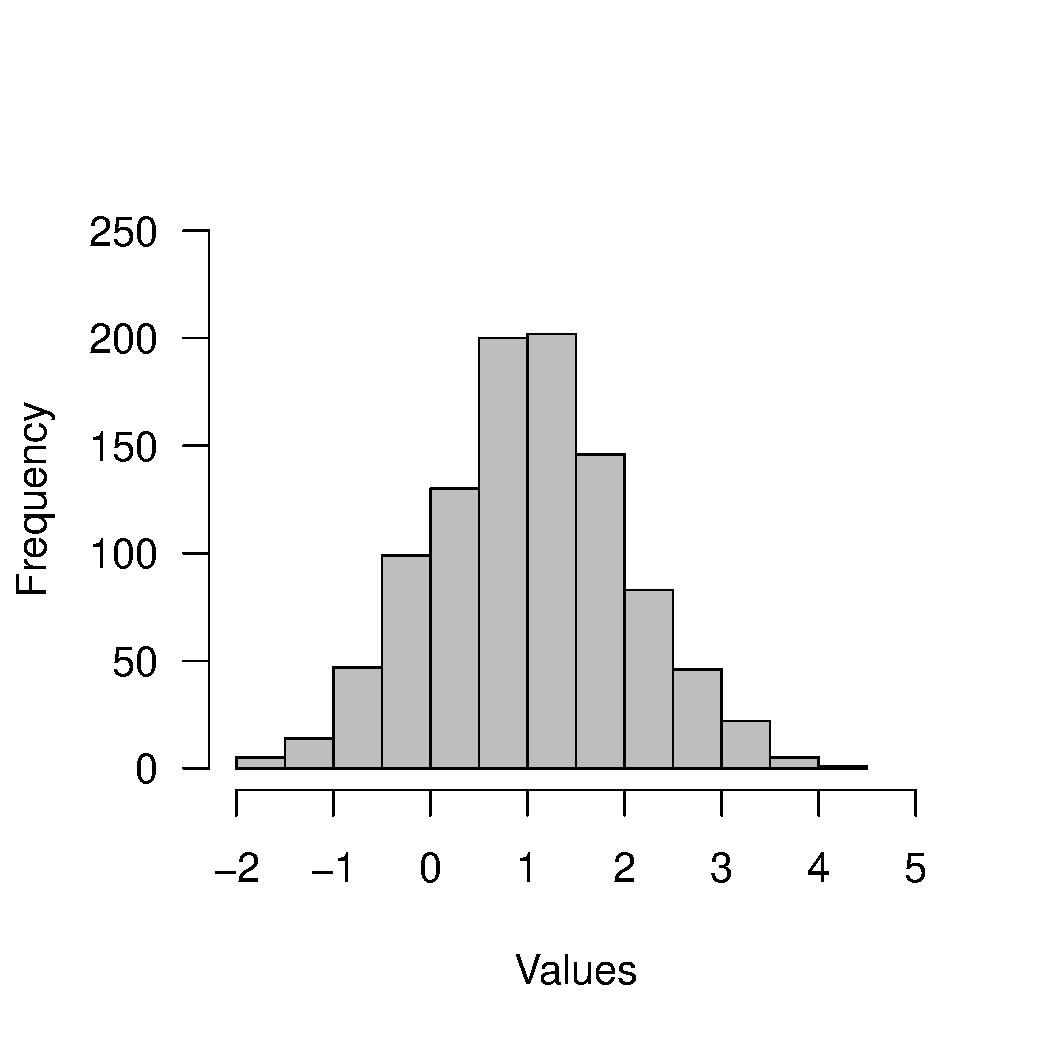
\includegraphics[width=\maxwidth]{figure/unnamed-chunk-3-1} 

\end{knitrout}

\subsection{Animating the Results}



\end{document}
